\documentclass[english]{article}
\usepackage[utf8]{inputenc}
\usepackage[T1]{fontenc}
\usepackage{color}
\usepackage{mdframed}
\usepackage{amsmath}
\usepackage{amssymb}
\usepackage[a4paper, total={6in, 8in}]{geometry}
\usepackage{graphicx}
\usepackage{natbib}
\usepackage[hidelinks]{hyperref}
\setlength{\headheight}{20pt} 

\definecolor{lightyellow}{RGB}{250,250,245}
\newcommand{\takeaway}[1]{
\begin{mdframed}[backgroundcolor=lightyellow] 
\textbf{Takeaway} #1 
\end{mdframed}}

\newcommand{\TODO}[1]{{\color{red} TODO - #1}}

\begin{document}

\title{Notes on NAACL 2018}

\author{Zining Zhu \footnote{Winterlight Labs + University of Toronto, \url{http://ziningzhu.me/2018/06/05/NAACL2018}, \texttt{zining.zhu@mail.utoronto.ca} }}
\date{New Orleans, Louisiana, June 5, 2018}

\maketitle

\vspace{1cm}

\tableofcontents


\section{Friday 0601}

\subsection{T1: Modelling NL, programs, and their intersection}

\paragraph{Speakers} Professors Graham Neubig and Miltos Allamanis for sharing the slides.

\subsubsection{Programming language vs natural language}
- a lot of similarities between programming languages and domain-specific languages \\
- data sources available. e.g: Stack Overflow\\
- Categories of data: intent, written intent, code snippets, doc strings, comments, diff messages\\


\subsubsection{Methods for mapping code to natural language}
\begin{itemize}
	\item Translation: (natural language description). Methods: machine translation, CNN + attentions, etc.
	\item Code summarization. e.g: Iyer et al "summarizing source code using a neural attention model". e.g: predict method names
	\item Convolutional neural attention models with attention mechanisms (which decide whether copy or summarize, similar to pointer-generator network)
	\item Incorporating the execution results to evaluate quality of generated programs
	\item Programming by demonstration...?
	\item Semantic parsing from Q-A pairs. Weak supervision is easier to create (e.g: for generating SQL. Zhong+17, Clarke+10)
\end{itemize}

\subsubsection{Program generation: map from language to code}
\begin{itemize}
	\item Machine translation, but with clear destination syntax rules
	\item Historical methods: rule-based transformations, grammar-based models, neural models. Following talks about neural approaches.
	\item How to take advantages of features of code? e.g: copy variable names. (word-level or character-level, or tree-level (Dong+16)) e.g: Top-down generation of CFG rules
	\item Also possible to generate codes from coarse-to-fine level (Dong+18). First predict the sketches, and then codes
	\item Code synthesis with natural language guidance (Polosukhin+18)
	\item Reconstruction loss: supervision without execution (Yin+18). Can use VAE formulation
	\item Code search: output API calls, Gu+2016 
\end{itemize}

\subsubsection{Modeling natural language aspects of source code}
\begin{itemize}
	\item Predict variable names
	\item Type inference. This has a lot to do with intelligent IDE
	\item If we represent program structures as a graph. 
\end{itemize}

\subsubsection{Modeling communicative aspects of software projects}
\begin{itemize}
	\item Model discussion topics: what are they talking about?
	\item Measuring the complexity of languages / codes (meaningful to Q-A sites)
	\item sentiment analysis for software (Lin+18)
\end{itemize}


\subsection{T3: Scalable construction adn Reasoning of Massive KB}
\paragraph{Speakers} Professors Xiang Ren, Nanyun Peng, and William Yang Wang

\textbf{Intro}
\subsubsection{Use cases for Text to Structure} 
TripAdvisor travel review, precision medicine (read the PubMed papers), search engines. 

Prior art: extracting structures with repeated human effort. Works pretty well but hard to scale.

Our method: effort-light structure extraction. Knowledge -> text corpus -> corpus-specific models -> structures.

Difficulty: aparsity of "matchable" (incomplete knowledge bases, low-confidence matching), 

\subsubsection{Methodology}
\paragraph{The tasks}
\begin{itemize}
	\item Data-driven text segmentation
	\item Learning corpus-specific model
	\item Structures from the unlabeled data
\end{itemize}

\subsubsection{Part 1: Recognize entities of target types in text}
Traditional NER systems: sequence model training. e.g: Stanford NER, Illinois name tagger, IBM Alchemy APIs

Training sequence models is slow + heavy reliance on corpus-specific human labeling.

Weak-supervision systems: pattern-based bootstrapping
(send several examples as "seeds"). Problem: can include wrong patterns.
\begin{figure}[h]
	\centering
	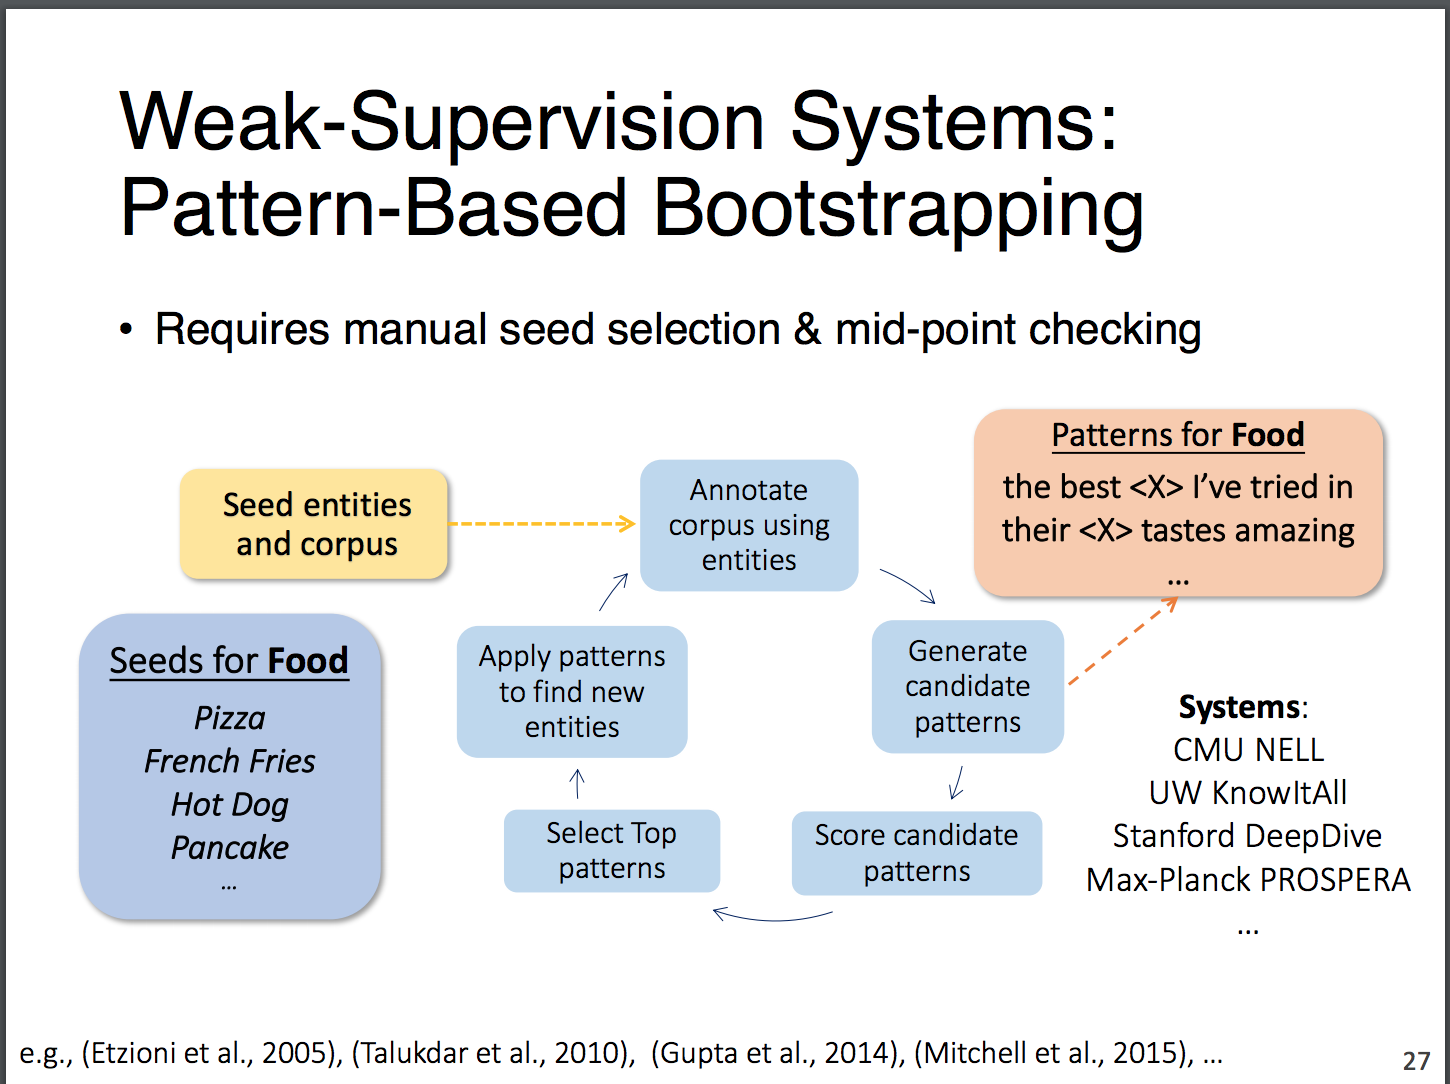
\includegraphics[scale=0.5]{fig0601/weak-supervision-ppt}
\end{figure}

\paragraph{Leveraging distance supervision.}
1. Detect entity names from text\\
2. Match name strings to KB entities.\\
3. Propagate types to the un-matchable names

LImitations:
\begin{itemize}
	\item Context-agnostic type prediction.
	\item Sparsity of contextual bridges (people describing the same things using different terms). This results in inefficient type propagation. 
\end{itemize}
Example: ClusType approach (KDD '15): type propagation + relation phrase clustering at the same time.\\
Smoothness assumption: if two nodes are similar saccording to the graph, then their type labels should also be similar.  

Two relation phrases should be grouped together if: (1) similar string; (2) similar context; (3) similar types for entity arguments. --> Multi-view clustering.

From coarse-grained typing to fine-grained entity typing:
For a clean mention, its "positive types" should be ranked higher than all its "negative types". 

Hierarchical type inference (Ren et al EMNLP '16)

Partial label embedding (PLE, KDD '16)\\

Comparison: WSABIE (Google ACL '15)
Predictive Text Embedding (MSR)

\paragraph{Prior works}
e.g: CoType approach (WWW '17)
Co-embedding for typing entities and relations

\subsubsection{Part 2: Joint extraction of typed entities and relations}
How to leverage other knowledge, such as the distributional statistics of characters and words, and annotations for other tasks and other domains, and the linguistics and problem structures, to combat the problem of inadequate supervision and conduct low-resource information extraction.

\paragraph{Traditional NER method} sequence tagging models, hand-engineering features

\paragraph{Neural NER models} e.g: RNN for representation. 

\paragraph{Distributional similarity of words}
Why not perform joint learning of word embeddings and NER?
\begin{figure}[h]
	\centering
	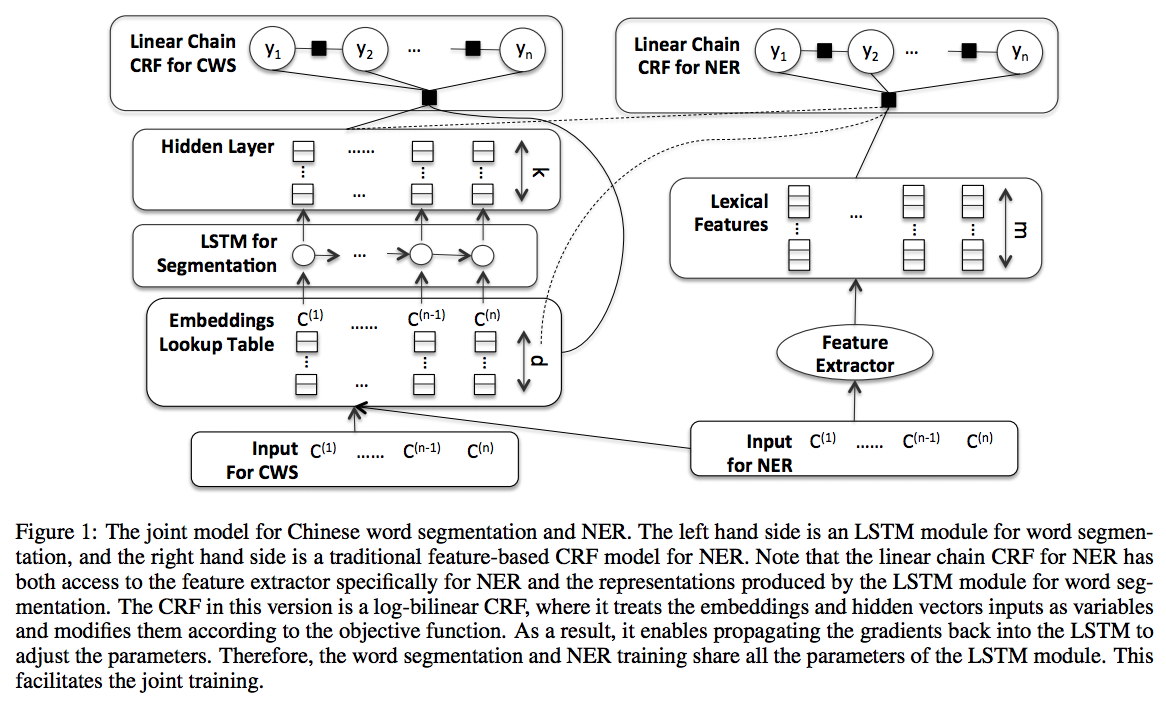
\includegraphics[scale=0.8]{fig0601/peng2015NER}
\end{figure}

e.g: chinese word boundaries

\paragraph{Sharing high-level representations} (Peng and Dredze, 2016)
\begin{figure}[h]
	\centering
	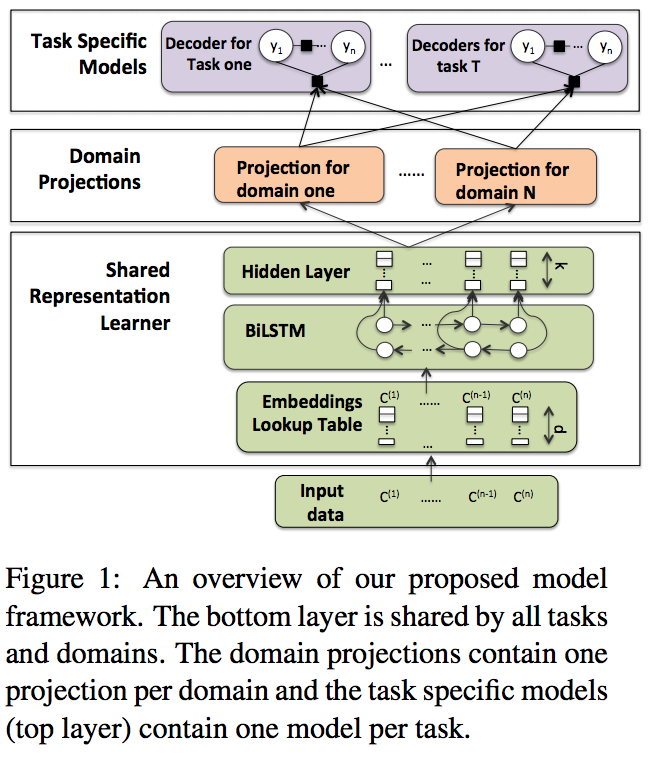
\includegraphics[scale=0.6]{fig0601/peng2016multi-task}
\end{figure}

\paragraph{Domains for languages}
Multi-task multi-domain learning. (Peng and Dredze, 2017) \\
Task-specific models  -- domain projections -- shared representation learner

\paragraph{How to build NER for a new language} using (1) comparable corpora (e.g. wikipedia) and (2) English NER tagger? (Want, Peng and Duh, 2017) \\
Motivation: learn a bilingual word embedding\\

Two approaches:
\begin{itemize}
	\item Fixed embeddings
	\item multi-task training
\end{itemize}

\paragraph{Encoding linguistic structures to improve}
e.g: cross-language N-ary relation extractions. Problem: hard to define the shortest path. Also, we are not allowed to go across the boundaries.
(Peng et al, 2017) representation learning framework.

$\bullet$ Goal; want to construct a representation learner, that captures difference types of dependencies over an \emph{acyclic graph}.

$\bullet$ Previous approaches: graph neural network, tree neural network, etc.
Problem: RNNs are expensive, and that information does not propagate to distant nodes.

$\bullet$ (Peng et al, 2017) cross-sentence n-ary relation extraction with graph LSTMs (in comparison to chain LSTM, there is one more forget gate per dependency)

$\bullet$ Multi-task learning from the shared representation learning


\subsection{Part 3: Recent advances in knowledge base reasoning}

\paragraph{Motivations} Knowledge Graphs are not complete. Missing links, etc.\\

$\bullet$ Knowledge graph supports various applications: structured search, QA, ASR, relation extraction, summarization, etc.

$\bullet$ Goal: complete the knowledge graph automatically (leveraging existing knowledge graph).

\paragraph{Path-based reasoning}
Why do we need path-based algorithms? (but not neural network embeddings) Explainability!
\begin{itemize}
	\item Path-ranking algorithm (Lao et al 2011) First random walk with restarts, then do LogReg to rank different paths (make paths leading to the correct destinations have higher weights)
	
	\item ProPPR, Wang et al 2013 PhD thesis and Want et al 2015. Generalizes PRA with recursive probabilistic logic programs. May use other relations to jointly infer this target relation.
	
	\item Subgraph feature extraction, Gardner et al 2015
	
	\item Chains of reasoning. Das et al 2017. PRA to derive path, then use RNNs to perform reasoning of the target relation.
	
\end{itemize}


\paragraph{Embedding-based reasoning}
Related method. (Robust and scalable)
\begin{itemize}
	\item RESCAL, Nickel et al, 2011. Tensor-based factorization. Head entity - tail entity - relation tensor. $Y=EWE^T$
	\item TransE, Bordes et al, 2013. If you have the initial embedding, and you add the relation to the head entity, you should get close to the target tail entity.
	\item Neural Tensor Network, Socher et al, 2013
	\item TransR / CTransR Lin et al 2015
	\item Complex Embeddings, Trouillon et al, 2016
	\item Poincar{\'e} embedding. Get out of the Euclidean space. Learn hierarchical KB representations by looking at hyperbolic space. $$d(u,v) = arcosh(1+2\frac{||u-v||^2}{(1-||u||^2)(1-||v||^2)})$$
	\item ConvE (Detters et al, AAAI 2018) learn entities with CNN. Reshape head and relation embeddings into "images".
\end{itemize}


\paragraph{Bridging path-based and embedding-based reasoning}: DeepPath, MINERVA, and DIVA\\
\begin{itemize}
	\item RL for KB reasoning: DeepPath (Xiong et al 2017 EMNLP). Path finding as a MDP. Train RL agent to find paths. Represent KG with pretrained KG embeddings. Use he learned paths as logical formulas.
	\item MINERVA: Das et al ICLR 2018. Go for a walk and arrive at the answer.
	\item DIVA: Variational KB reasoning. Inferring latent paths connecting entity nodes.
\end{itemize}

Sidenote: RL is a general purpose framework for decision making. 



\subsection{T5: Socially Responsible NLP}
\paragraph{Speakers} Professors Yulia Tsvetkov, Vinodkumar Prabhakaran, Rob Voigt \\
(ref: CMU CS11830)

$\bullet$ Be careful: nobody is expert simultaneously in all of the sociology + psychology + linguistic + CSC + ML + statistics. 

\subsubsection{Ethics in NLP: foundations}

$\bullet$ What is ethics? About doing the good / right things. Problem: sometimes cannot define good / bad properly. 

$\bullet$ Another example: the chicken classifier (hen -> egg farm; roster -> meat farm)

$\bullet$ Ethics versus law

$\bullet$ Identify a range of problems / questions we should ask when building NLP systems.

$\bullet$ E.g: the A.I. "Gaydar"

\subsubsection{Technical Aspects}
\paragraph{Humans are the "natural" in NLP}
In a way, NLP is human subjects research.

$\bullet$ Self-selection bias. e.g: who posts on Yelp

$\bullet$ Reporting bias. e.g: People do not necessarily talk about things in the world in proportion to their empirical distributions.

$\bullet$ (Jurgens et al ACL 17) Socioeconomic bias in language identification.

\subsubsection{Case study}

$\bullet$ The semantic of words contain inherent biases. e.g: the bias embedding test. Might be able to exclude some of them using fair learning. \\
/* Excluding gender differences from semantic embeddings is possible, but how about languages like French, where gender difference is encoded as syntactic rules? */


\subsubsection{Test}

$\bullet$ Should care about whether the task is beneficial to the people involved. The purpose is not going to build "gaydar" or "tell the race of driver based on the police officer's speeches". 

$\bullet$ There can be multiple causes for an effect. We should not give blatant judgements without fully assessing them. For example, among those pulled over \emph{only for minor ticketing}, African Americans receive more tickets for minor car damages. This could due to biases in police officers. This could also due to their economic status (less frequently go to repair the cars once damaged? ), etc.

$\bullet$ There are complicated reasons behind these problems. Be careful when organizing sentences, etc.

$\bullet$ Extension: CS294 fair learning. Also Graeme Hirst's CSC D03 (social impacts of ML).

\takeaway{People are focusing more on the fairness of machine learning. ML researches should take more social responsibilities: Present the researches in an explainable manner, and explore the indications of the researches.}

\section{Saturday 0602}


\subsection{Information Extraction 1}
Empire A

\subsubsection{\cite{Gupta2018Joint} Joint bootstrapping machines for high confidence relation extraction}
\begin{itemize}
	\item Challenge: semantic drift
	\item solution: BREX. Use entity and template seeds jointly
\end{itemize}

\subsubsection{\cite{Wang2018Label-Aware} Label-aware double transfer learning for cross-specialty medical NER}
\begin{itemize}
	\item Problem: NER from electronic medical records
	\item Framework: See figure
	\item Optimization goal: $\mathcal{L_{crf}} + \alpha \mathcal{L}_{La-MMD} + \beta \mathcal{L_p} + \gamma \mathcal{L}_{\text{regularizer}}$, CRF + La-MMD loss + parameter similarity loss + regularization.
\end{itemize}
\begin{figure}[h]
	\centering
	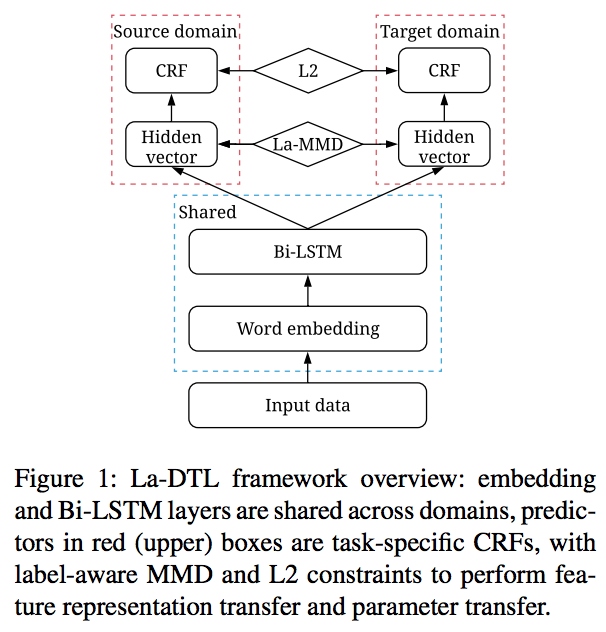
\includegraphics[scale=0.9]{fig0602/LA-MMD}
\end{figure}

\subsection{Morning Poster:  Discourse and Pragmatics 1}
Elite Hall A

\subsubsection{\cite{Schulz2018Multi-Task} Multi-task learning for argumentation mining in low-resource settings}
\begin{itemize}
	\item Task: argumentation mining: segment a text into argumentative and non-argumentative components and identify them. 
	\item: Method: MTL (training a system to solve several conceptually different AM tasks jointly) improves performance over learning in isolation.
\end{itemize}

\subsubsection{\cite{Fu2018Natural} Natural answer generation from heterogeneous memory}
\begin{itemize}
	\item Task: Seq2seq sentence-in sentence-out QA
	\item Problem: Information come from heterogeneous information sources.
	\item Proposed model: Incorporate three components in the decoder hidden state: $h_n$, predicting words from the vocabulary, $h_k$: key pointer, $h_v$, value pointer. Use a gate to mix them, so the resultant network is optimizable through back propagation.
\end{itemize}


\subsubsection{\cite{Baly2018Integrating} Integrating stance detection and fact checking in a unified corpus}
\begin{itemize}
	\item Problem: (part of) fact checking. Decide whether a claim is relevant to a document, and decide whether the document supports the claim.
	\item This work describes the corpus and evaluated using some algorithms someone used in competition. Also referring to their another work next Monday: \cite{Mohtarami2018Automatic}
\end{itemize}

\subsubsection{\cite{Novikova2018RankME:} RankME: reliable human ratings for natural language generation}
\begin{itemize}
	\item Problem of human rating for NLG: consistency, distinct criteria, relative assessment, etc.
	\item Solution: rank-based Magnitude Estimation (RankME), with relative ranking on continuous scale.
	\item How to assess the rating? Intra-class correlation coefficient (ICC)
\end{itemize}


\subsubsection{\cite{Mitcheltree2018Using} Using aspect extraction approaches to generate review summaries and user profiles (Airbnb)}
\begin{itemize}
	\item Task: Aspect extraction. Subtasks: (1) extract a representative sentence from a set of listing-specific reviews for a number of pre-defined aspects (e.g: cleanliness, location). (2) The suitability of aspect embeddings to represet guest profiles.
	\item Comparison between KMeans and ABAE (Attention-based aspect extraction. He et al., 2017), both of which are much better than LDA in these aspect extraction tasks.
\end{itemize}


\subsection{Machine Learning 1}
Empire A

\subsubsection{\cite{Rei2018Zero-Shot} Zero-shot sequence labeling: transferring knowledge from sentences to tokens}
\begin{itemize}
	\item Task: give each token in a sentence a label (of what?), without telling the model how to predict
	\item Previous work to visualize LSTMs using e.g., attention weights, usually work on only a few data samples, and qualitatively.
	\item Method: First train a word LSTM (with attentions) on the classification task (e.g. the uncertainty prediction task), and that attentions show which tokens are the most important. This is the golden annotation $y$. Also the supervised learning "upper bound" baseline.
	\item Where does the zero-shot learning come from? Given this trained network, perform a "backprop from pseudo-label" operation, assuming the pseudo-label is 0. Calculate the gradients at the words. For those whose labels are already 0, the gradients shall be small. Those words labeled as 1 should have large gradients. In this paper, this threshold is set to 1.5 deviation.
\end{itemize}
\takeaway{ The evaluation should be those of the supervised classifier's accuracies -- zero-shot learning can \emph{not} give this kind of per word accuracies. But visualizing the magnitude of gradients is a good idea to visualize LSTMs.}




\subsection{Machine Learning 2}
Empire A
\subsubsection{\cite{Benton2018Deep} Deep dirichlet multinomial regression}
\begin{itemize}
	\item Topic models. e.g. supervised topic models. What if the etadata are high-dimensional, structured, or may not directly relevant to modeling topics.
	\item Backbone: LDA. Change to DMR: sample from document-specific priors. 
	\item From DMR to deep DMR
	\item Trained with Gibbs sampling.
\end{itemize}

\subsubsection{\cite{Rooshenas2018Training} Training structured prediction energy networks with indirect supervision}
\begin{itemize}
	\item Structured prediction
	\item Parameterize energy function over y as a DNN -> can find the min of E using gradient descent.
	\item Supervised learning: Structured SVM (Belanger and McCallum, 2016)
	\item Indirect supervision 
	\item Rank-based training
\end{itemize}


\subsubsection{\cite{gallagher2016anchored} Anchored correlation explanation: topic modeling with minimal Domain Knowledge}

\begin{itemize}
	\item How to do topic modeling with thousands of information bottleneck?
	\item LDA is a a generative topic model. Goods and bads of generative modelings.
	\item Topic model that learns topics through information-theoretic criteria.
	\item CorEx (total Correlation Explanation): a topic is a binary latent factor. Goal: find factors that make words conditionally independent. 
	$$ \min_Y TC(W_1 .. W_n | Y) = \min_Y D_{KL} \left ( p(w_1, .. w_n | y) || \Pi_i p(w_y | y) \right )$$
	$TC(W|Y)=0$ iff the topics "explain" all the dependence (total correlation). Here comes the Correlation Explanation name.
	\item Then rewrite the objective as mutual information
	$$\min_Y \Sigma_i I(Y_j : W) - \Sigma_i \alpha_{i,j} I(W_i; Y_j)$$
	where $\alpha_{i,j} = \frac{I(W_i : W_j | Y_{k \neq j})}{I(W_i : Y_j)}$, which is the unique information in $Y_j$ about $W_i$
	
	Then transform a combinatorial to a continuous optimization

	\item Extensions: (1) hierarchical CorEx; (2) semi-supervised learning.
	\item Anchored CorEx objective is exactly maximizing the information bottleneck.
\end{itemize}


\subsubsection{\cite{zhang2017aspect} Aspect-augmented adversarial networks for domain adaptation }

\begin{itemize}
	\item Problem: Transfer learning, but both source and target classifiers operate over the same domain.
	\item Method: Learn a document-level representation that is hard to tell the domain, but easy to tell the class label.
	\item The encoder contains:
	A CNN per sentence; Improve adversarial training by reconstruction.
	\item Apply relevance score using a small set of keyword rules. 
\end{itemize}
\begin{figure}[h]
	\centering
	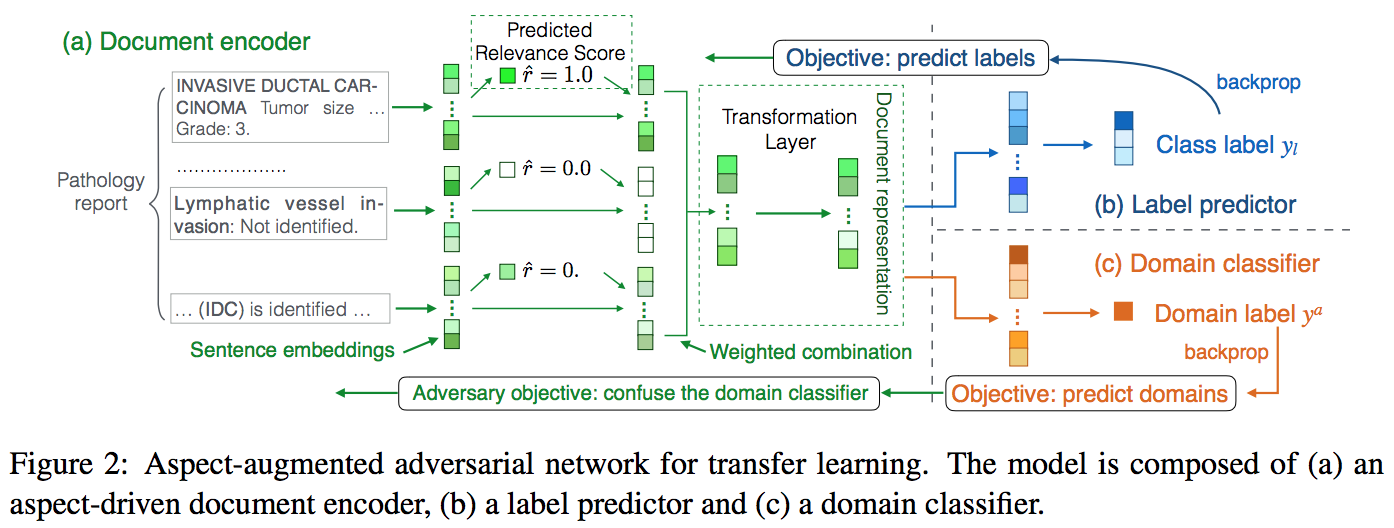
\includegraphics[scale=0.6]{fig0602/zhang2017aspect}
\end{figure}


\subsection{SRW highlights}
Empire C

\subsubsection{\cite{Ezeani2018Igbo} Igbo diactritic restoration using embedding models}
\begin{itemize}
	\item Igbo language: more spoken than written, and low-resource for NLP. (mostly south-eastern Nigeria)
	\item Problem: diacritic ambiguity (same wordkey, but different meanings)
	\item Embedding projection: align English embedding to Igbo language, using an alignment dictionary.
	\item Diacritic retoration proces: during evaluating candidate instances, choose the one with the maximum (cosine?) similarity in the embedded vector.
\end{itemize}

\subsubsection{\cite{Acharya2018Towards} Towards generating personalized hospitalization summaries}
\begin{itemize}
	\item Problem: summarization
	\item Method: FIrst build concept graph via UMLs, extract physician / nursing concepts to include. Then simplify. Then Arrange event ordering.
\end{itemize}

\subsubsection{\cite{Shin2018Alignment} Alignment, acceptance, and rejection of group identities in online political discourse}
\begin{itemize}
	\item Trump and Clinton supporters tend to use and align pronouns differently.
	\item Their rhetorical words are not substantially different.
\end{itemize}
\section{Sunday 0603}

\subsection{Morning Keynote: The moment when the future fell asleep}
Professor Kevin Knight
\paragraph{Decipher}
Deciphering of some ancient languages.\\
Decipherment is the original NLP problem.

\paragraph{Generative model for cipher}
\begin{figure}
	\centering 
	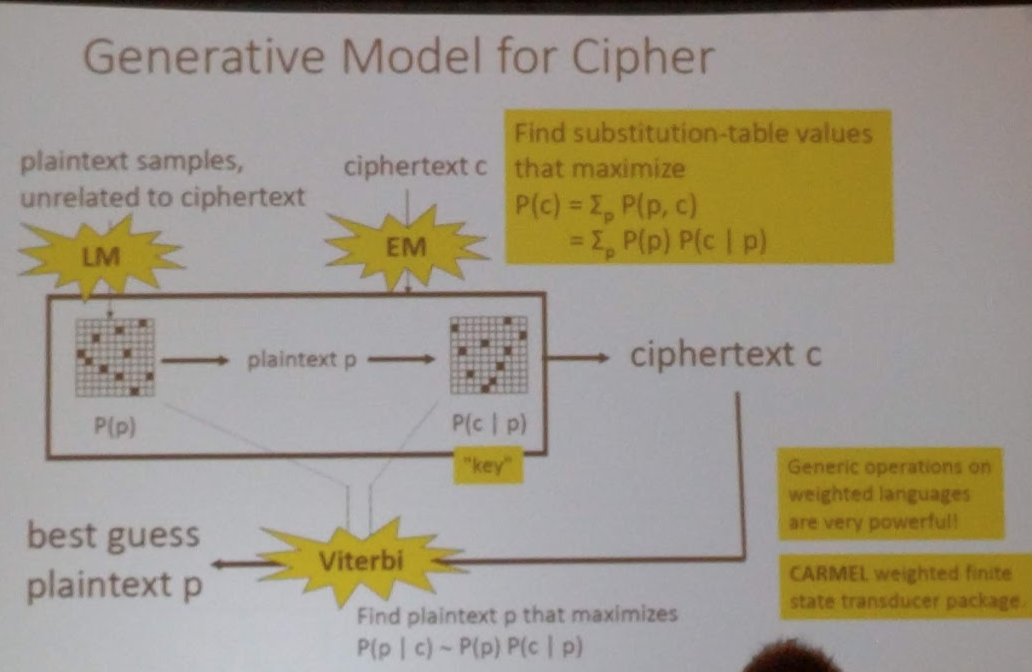
\includegraphics[scale=0.8]{fig0603/kn-cipher-model}
\end{figure}

\paragraph{Recent works}
\begin{itemize}
\item Pixel image -> OCR + decipher in the system -> plain text. No supervision segment and clustering. After that, apply noisy-channel methods with plaintext language model.
\item Zodiac cihpers: Z340, Z32, Z13
\item Improve on the plaintext language models might lead to lower decipher error.
\end{itemize}

\paragraph{Poetry generation}
\begin{itemize}
	\item Can generate poets e.g.: Ghazycininejad, Shi, Choi, Knight EMNLP 2016
	\item Hafez: an interactive poetry generation system (Ghazvininejad et al. ACL demo 2017)
\end{itemize}
\begin{figure}[h]
	\centering 
	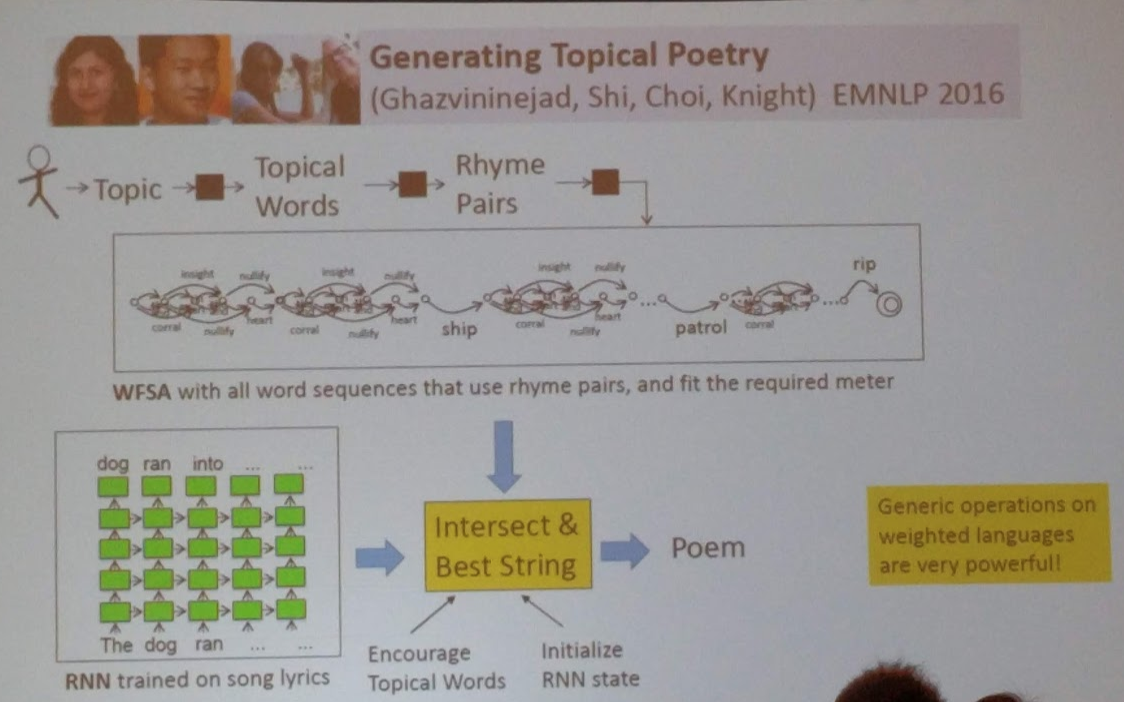
\includegraphics[scale=0.8]{fig0603/kn-generate-poetry}
\end{figure}

\paragraph{RNNs for storytelling}
\begin{itemize}
	\item How to memorize a random 60-bit string?
	\item RNNs as weighted language recognizers \cite{Chen2018Recurrent}
	\item Does string-based NMT learn source syntax? (EMNLP 2016)
	\item Why neural translations are the right length? (EMNLP 2016). 
	\item Towards controllable story generation? (Peng et al., NAACL 2018 storytelling workshop) 
	\item Paper anstract writing through abstract mechanism (Want et al, ACL 2018)
	\item Neural poetry translation \cite{Ghazvininejad2018Neural}
\end{itemize}

Why do automatic outputs look so different (to us) than what was trained on?

\paragraph{Conclusions}
Still a long way to go. NLP for entertainment, commerce.


\subsection{Morning Posters}

\subsubsection{FEVER: a large scale dataset for fact extraction and verification \cite{Thorne2018FEVER:}}
\begin{itemize}
	\item A dataset containing 185,000 facts. Each wiki passage (?) has (humanly labeled) several claims (true or false).
\end{itemize}

\subsubsection{Efficient sequence learning with group recurrent networks \cite{Gao2018Efficient}}
\begin{itemize}
	\item Sequence learning task.
	\item Divide the hidden layer into two parts, so that computation is more efficient.
	\item Mix two parts of the hidden representation by the rearrange() function, so that the inter-group correlation can be considered more.
\end{itemize}

\subsubsection{Embedding syntax and semantics of prepositions via tensor decomposition \cite{Gong2018Embedding}}
\begin{itemize}
	\item Train a word embedding considering the tensor decomposition and preposition embeddings.
	\item The loss function contains ALS model term and the bias scalar parameters.
\end{itemize}

\subsubsection{Semi-supervised event extraction with paraphrase clusters \cite{Ferguson2018Semi-Supervised}}
\begin{itemize}
	\item First cluster the articles. Then identify "easy" events (after running a pre-trained supervised system on all sentences). Select most likely triggers for "hard" mentions.
\end{itemize}




\subsection{Machine Learning 3}
Empire A
\subsubsection{Deep generative model for joint alignment and word representation \cite{Rios2018Deep}}
\begin{itemize}
	\item Optimize the variational lower bound of the marginal likelihood of a sentence pair: $P_\theta (x_i^m, y_j^n | m, n)$ where $x_i^m$ and $y_j^n$ are word observations in languages 1 and 2 respectively.
\end{itemize}


\subsubsection{Evaluating the stability of embedding-based word similarities}
\begin{itemize}
	\item Cosine similarities are not satable. They have biases w.r.t corpus from which the word2vec are trained.
	\item Question: what do embeddings represent? They measure the properties of a curated corpus, not the word themselves.
	\item Two views of embeddings: downstream-centered or corpus-centered. (This work focus on the corpus-centered view)
	\item The embeddings are calculated using LSA (latent semantic analysis + tf-idf using \texttt{sklearn}), SGNS (skip-gram with negative sampling), GloVe, and PPMI (positive point-wise mutual information). Each methods contain fixed, shuffled, and bootstrap settings.
	\item Measure the cosine similarity bound of 20 query words. Those with lower variances is more stable.
\end{itemize}

\takeaway{Should study from the methodology for designing experiments.}

\subsubsection{Learning word embeddings for low-resource language PU learning \cite{Jiang2018Learning}}
\begin{itemize}
	\item Problem: large datasets are required to train datasets. Might be hard to find this large of corpus for low-resource languages. (this project focus on those with low-resource, but not those very-low-resource languages)
	\item Problem: Sparsity of the co-occurrence matrix (>99\% of them are zero). Can be true zeros or missing entries (can co-occur but just has not in the given corpus)
	\item Motivation: word2vec use negative sampling, which only subsamples for some of the not mentioned.
	\item Propose a PU-learning framework for training word embedding. The learning alg deals wiht all negative pairs.
	\item Three components in the framework: 
	(1) Pre-processing (building the o-occurrence matrix -> scale counts by PPMI metric w.r.t [Levy '15]) 
	
	(2) PU-learning for matrix actorization: $A \approx W^T H$, where we try to optimize (using coordinate descent)
	(see paper for the equations)
	
	(3) Post-proessing. Average $w_i^T$ and $h_i$ to get the resulting word vector.
\end{itemize}


\subsection{Afternoon keynote: building innovative startups, products, and services -- personal insights}
Daniel Marcu (Amazon)
\begin{itemize}
	\item Hard to annotate all domains -- they are just too many of them. Very important therefore to enable domain adaptation.
	\item Commercial requirements usually forces us to be short-sighted.
	\item The most important lesson: We owe success to those people we worked with.
	\item Example of exploration in NMT structures.
	\item Important to know that the world is not just the pinnacle we focus on (e.g., in PhD). The world is the whole circle (big picture) -- much more than what you have been focusing on pushing.
	\item Q: expectation between tech people and marketing people. People might like to go hype; also scientists should not make overly promising claims.
	\item Some tasks are hard to evaluate. These will be what a lot of future projects work on. e.g: quality of Alexa communication.
\end{itemize}

\subsection{Afternoon Posters}
\subsubsection{Diverse few-shot text classification with multiple metrics \cite{Yu2018Diverse}}
\begin{itemize}
	\item Task: Few-shot learning in diverse tasks.
	\item Propose an adaptive metric learning approach that automatically determines the best weighted combination from a set of metrics obtained from meta-training tasks for a (new) few-shot task.
	\item Matrix-completion based task clustering
\end{itemize}

\subsubsection{Cross-lingual learning-to-rank with shared representations \cite{Sasaki2018Cross-Lingual}}
\begin{itemize}
	\item Task: For each query-document pair, learn a mapping. More specifically, a query CNN and a document CNN compress the query and document into a hidden embedding.
	\item Several models to learn transferrable knowledge between languages. A basic "cosine model" minimizes the cosine similarity between the query and document embeddings. This does not work well on low-resource languages.
	\item A deep model adds a MLP to learn a similarity score given the embedding. How to make this model work on low-resource setting?
	\item Parameter-sharing is the improvement. Use the query CNN and the MLP trained on a high-resource language, and fine-tune using a low-resource language.
\end{itemize}


\subsubsection{Are all languages equally hard to language-model? \cite{Cotterell2018Are}}
\begin{itemize}
	\item Hypothesis: inflectional morphology makes a language hard to model. LM performance negatively correlated with morphological counting complexity.
	\item Correlation disappears when modeling lemmata instead of forms.
	\item Different languages contain varying bits per (English) character.
	\item The comparison methods are the takeaways at the end of the day.
\end{itemize}


\subsection{Text Mining 1}
\subsubsection{Explainable prediction of medical codes from clinical text}
\begin{itemize}
	\item Task: the clinical coding problem
	\item Model: word embed -> CNN features -> attend (one for each label) -> classifier (Logistic Regression)
\end{itemize}

\subsubsection{Event-time extraction with a decision tree of neural classifiers \cite{reimers2018event}}
\begin{itemize}
	\item Temporal links annotations
	\item Problem: sparse annotation of event times.
	\item TLINK annotation: dense annotation of event times. (ACL '16)
	\item Temporal anchoring of events given complete documents.
	\item Dataset: TimeBank-EventTime Corpus
\end{itemize}

\subsection{Test of Time}
Empire B

\subsubsection{Remembrance of Aravind Joshi}
\begin{itemize}
	\item 1929 - 2017
	\item Centering: a framework for modeling the local coherence of discourse; the penn discourse treebank; tree adjoining grammars.
\end{itemize}

\subsubsection{BLEU}
\begin{itemize}
	\item ACL 2002, Kishore et al.
	\item "Bilingual Evaluation Understudy": compare short runs of candidate text against reference translations.
	\item Not necessary to match pair-wise
	\item All words are equally important: all you need is a tokenizer. Set up a brevity penalty BP:
	\[BP=\left\{ \begin{matrix} 1 \text{if c > r}  \\ e^{1-r/c} \text{otherwise} \end{matrix}  \right. \]
	\item Modified u-gram precision: average log with unit weights.
	\item BLUE = $BP \times exp(\sum_n w_n log p_n)$  where $p_n$ is the n-gram precision, and positive weights $w_n$ sum up to 1.
	\item Stunningly simple, surprisingly simple.
\end{itemize}

\paragraph{Retrospective}
\begin{itemize}
	\item Context: DARPA: slow and expensive for human evaluations; long pause in funding.
	\item Hard to sell in 2002: "quantity leads to quality". "Don't attempt to divine human judgment for every sentence. Rather, average out individual sentence judgment errors over a corpus."
	\item Polarization: people have polarized reviews towards BLEU.
	\item It is an understudy -- never meant to replace human judgments.
	\item Q: criticism that BLEU penalizes stylicism? A: wow the metrics actually understand language.
\end{itemize}

\subsubsection{Structured Perceptron}
\begin{itemize}
	\item EMNLP 2002, "Discriminative Training Methods for HMM", Michael Collins
	\item Background: structured prediction problems
	\item Dominant approach in the 1990s to do structured prediction as density estimation: model $p(x, y)$ or $p(y|x)$. e/g: Log-linear history-based models.
	\item Method: POS Tagging with HMMs
	\item Generalization bounds. (written in a PAC-style).
	\item Conclude: thoughts about learning and search.
	
	Approach 1: global training. e.g: CRF log-loss, max-margin
	
	Approach 2: Local training, etc., seq2seq
	
	\item Some hypotheses in 2002: (1) search is necessary for some structured prediction problems. (2) If you believe search is beneficial, then local normalization does not work. (3) Generalization bounds will be important in a scientific understanding of why / how machines learn. (see Dziugaite and Roy on PAC-Bayes for NN)
	
	Interesting to think about them.
\end{itemize}

\subsubsection{A sentiment Odyssey}
\begin{itemize}
	\item EMNLP 2002, Thumbs up? Sentiment classification using ML techniques by Bo Pang et al.
	\item Background: people start to use internet increasingly prevalently. Then sentiment analysis is increasingly important. Also the dataset sizes were pretty small.
	\item Released the imdb movie review dataset.
	\item Inspirational slide? Do something interesting but that might not be deemed interesting as considered by other people. Since most people here have done PhD they should know how to get out of it. 
\end{itemize}



\section{Monday 0604}

\subsection{Keynote: Google assistant or my assistant?}

\paragraph{Background}
Early conversation systems occurred in 1990s. Nowadays, however, the conversation systems stiil need a long way to go, because they should be multi-domained, and scalable (a lot of data-hungry methods are hard to scale).

\subsubsection{Task-oriented dialogue as a collaborative game}
A seeker and a provider agents. Human are usually the seeker, but machine could be seeker as well. Seeker has a goal but no access to solution. The provider has solutions but does not know the goal.

\paragraph{Provider} language understanding, state tracking, \{dialogue manager, response generator\} that queries the backend (action provider / knowledge bases).
\begin{itemize}
	\item Trained by RL aiming to optimize longer term dialogue reward (Levin et al, IEEE TASLP 2000, Singh et al AAAI 2000)
	\item Hierarchical RL for multi-domain dialogues (Peng et al, EMNLP 2017)
	\item Reward estimation (Su et al, ACL 2016)
\end{itemize}

\paragraph{Seeker} language understanding, dialogue state tracking, \{dialogue manager, response generator\} that interacts with the scenario.
\begin{itemize}
	\item usually termed as "user simulators". \item e.g: seq-to-seq models; 
	\item probabilistic, agenda based \cite{Shah2018Neural}
\end{itemize}

\paragraph{Crawl: machines talking to machines} \cite{Shah2018Bootstrapping} tries to produce dialogues that make sense to humans. 


\subsubsection{Dialogue system components attempts to solve challenges}

\paragraph{Conversational Language Understanding}
LSTM + attention?

How to Integrate conversation context?
Context vector, attention over history, time decay attention (Su et al, 2018 NAACL)

Challenge: scaling CLU to new verticals.
\begin{itemize}
	\item Zero-shot learning using slot tag and description embeddings as additional input during parsing (Bapna et al, Interspeech 2017)
	\item Train on target (LeFevre et al, Interspeech 2010)
	\item Test on source (Jabaian et al, ICASSP 2011)
	\item Joint learning on source and target (He et al, ICASSP 2013)
	\item Cross-lingual embeddings (Upadhyay et al, ICASSP 2018)
\end{itemize}

\paragraph{Referring expression resolution for situated dialogues}


\paragraph{Dialogue state tracking}
Agent's estimate of the user's goal(s) based on the dialogue history. Research on DST has been fostered by the dialogue state tracking challenges:
\begin{itemize}
	\item Delexicalised RNNs 
	\item Neural belief tracker 
	\item End-to-end memory networks for DST
	\item Recent pointer networks (Xu and Hu, arXiv 2018)
	\item Simulated datasets focus on entities that were not previously observed
	\item (Rastogi et al, IEEE ASRU 2017) Focus only on the relevant set of slot values
\end{itemize}

Accuracy and scalability are important, but efficiency is important too!
Hierarchical recurrent neural network  (Gupta et al, INterspeech 2018)
(Rastogi et al, SigDial 2018) that halved the parameter.

\subsubsection{End-to-end learning}
\paragraph{e2e dialogue with deep RL}
\begin{itemize}
	\item Component-wise training benefits from additional data for each component
	\item Supervised learning (Li et al ICASSP 2017, Bordes et al ICLR 2017)
	\item RL (Williams et al ACL 2017, Dhingra ACL 2017)
	\item Eng-to-end dialogue models with human teaching (poster at NAACL 2018)
\end{itemize}

\subsubsection{Other interesting topics}
\begin{itemize}
	\item Diverse in-domain dialogue data
	\item scaling to new domains / languages 
	\item integrating context
	\item scalable multi-domain state tracking
	\item learning about users
	\item Understanding and tracking with complex / compositional representations
	\item Generating multi-modal content
	\item Situated, multi-modal dialogues
	\item Latent understanding
\end{itemize}


\subsection{Morning posters}

\subsubsection{Deconfounded Lexicon induction for interpretable social science \cite{Pryzant2018Deconfounded}}
\begin{itemize}
	\item Need to mae social models transparent and interpretable. Formalize as" induce a lexicon that is predictive of a set of target variables yet uncorrelated to a set of confounding variables.
	
	Formally, look for L that maximizes informativeness coefficient: 
	\[\mathcal{I}(L) = \mathbb{E} [Var [\mathbb{E}[]Y|L(T), C  | C]] \]
	\item So they are monitoring the coefficient, but not optimizing it. The optimization is through an adversarial selector.
	\item Two deep learning algorithms for this task. 
\end{itemize}

\takeaway{The induced lexicons reminds me of anchor variables (Halpern et al)}

\subsubsection{Learning to rank Q-A pairs using hierarchical RNN with latent domain clustering}
\begin{itemize}
	\item Train hierarchical RNN, then cluster the latent dimensions
	\item Then incorporate each latent vector by the \emph{similarity} of it and all cluster topic vectors. 
	\item Interestingly, the latent topic cluster does not agree with the human clustering. I think this is reasonable -- you can't ensure that neural networks learn things exactly in the euclidean space.
\end{itemize}

\subsubsection{Supervised and Unsupervised transfer learning for question answering \cite{Chung2018Supervised}}
\begin{itemize}
	\item Model: memory networks. Use CNN to process the embeddings.
	\item For the supervised part: fine tune the upper network layers, or the whole networks, even including the embedding networks.
	\item For the unsupervised part: self-train bootstrapping.
	\item Dataset: Multiple choice QA.
\end{itemize}
\takeaway{This is an example where direct fine-tune transfer learning works. It is understandable that multiple choice QA knowledge are easy to transfer than other tasks like translation or classification.}

\subsubsection{Deep communicating agents for abtractive summarization\cite{Celikyilmaz2018Deep}}
\begin{itemize}
	\item Agent model: pointer network (seq2seq) for abstractive summarization.
	\item One paragraph per agent. Break down the difficult long text reading problem down to multiple agents.
	\item MLE loss: $L_{MLE} = -\sum_{t} log p(y_t | t_{1..t-1}, d)$. Try to make the predicted next word as close to the next ground truth word as possible.
	\item Semantic cohesion loss: $L_{sem} = \sum_{q} cos(s_q, s_{q-1})$. This encourages the generated sentences to be coherent with the previous sentence.
	\item Also contains an RL loss:  $L_{RL} = (r(\tilde{y}) - r(\hat{y})) \sum_t logp(\hat{y}_t | \hat{y}_{1..{(t-1)} , d})$. How are the reward decided? Self-critical approach. It is calculated by comparing the similarity between generated sentence and the ground truth.
	\item Putting the loss together: $L_{mixed} = \gamma L_{RL} + (1-\gamma) L_{MLE}$
	\item Evaluate using incremental ROUGE scores, considering the intermediate rewards.
\end{itemize}
\takeaway{So in many NLP works the reinforcement learning rewards refer to the one calculated upon reaching the end of a passage. In robotics setting RL loss corresponds to the end of an epoch. Note this difference.}

\subsubsection{Key2Vec \cite{Mahata2018Key2Vec:}} 
\begin{itemize}
	\item Procedure: Fasttext-skipgram
\end{itemize}

\subsubsection{Unsupervised keyphrase extraction with multipartite graphs \cite{Boudin2018Unsupervised}}
\begin{itemize}
	\item A multipartite graph: nodes from each group does not connect to each other.
	\item Adjust the weights of graph edges by some metrics w.r.t the entries.
\end{itemize}

\subsubsection{Estimating summary quality with pairwise preferences \cite{Zopf2018Estimating}}
\begin{itemize}
	\item Set up generated preferences as games: the better sentences are more likely to win the game.
	\item Compute Bradley-Terry scores: $p(s_x > s_y) = \frac{u(s_x)}{u(s_x) + u(s_y)}$. Now you have a list of preferences.
	\item Value of a summary (collection of sentences): $v(S) = \sum_{i}^{|S|} w_i u(s_i)$
	\item Automatically generating preferences (refer to paper for details)
	\item Using additional automatically generated labels can further improve accuracy.
\end{itemize}

\subsubsection{Which scores to predict in sentence regression for text summarization?\cite{Zopf2018Which}}
\begin{itemize}
	\item Recall is biased towards long sentences.
	\item Ordering according to prevision leads to better summaries.
	\item Takeaway: better select sentences according to ROGUE precision in summarization tasks.
\end{itemize}

\subsection{Generation 3}
Empire C
\subsubsection{Interpretable charge predictions for criminal cases}
\begin{itemize}
	\item Learning to generate court views from fact descriptions \cite{Ye2018Interpretable}
	\item Overview: charge prediction. Input: fact description in a criminal case. Output: charge label (e.g. drunk driving, intentional injury, etc.)
	\item Previous work lack interpretability
	\item What is court view? A written explanation from judges to interprete the charge, including rationale and charge label (only rationale generation this paper).
	\item High quality rationale? (1) Should contain relevant details; (2) should be charge-discriminative.
	\item Model: label-conditional seq2seq model. Bi-LSTM with attention. 
	\item How is the label-conditional work? The label is predicted using encoder attentions. Then the predicted label is passed as an additional input into every step of the decoder.
\end{itemize}


\subsubsection{Delete, Retrieve, Generate: a simple approach to sentiment and style transfer \cite{Li2018Delete}}
\begin{itemize}
	\item Text attribute transfer
	\item Previous work example: adversarial content saparation: (Shen et al 2017, Fu et al 2018)
	\item Proposed method: (based on seq2seq)
	
	(1) Delete the words most indicative to the sentiment (see paper for details)
	
	(2) Retrieve: decide what words to insert into context.
	
	(3) Generate: 
	
	\item Comparison models: TemplateBased, DeleteOnly, DeleteAndRetrieve

\end{itemize}


\subsubsection{Adversarial example generation with syntactically controlled paraphrase networks \cite{Iyyer2018Adversarial}}
\begin{itemize}
	\item Adversarial examples generation for images (Goodfellow 2015 ICLR)
	\item Lexical adversaries (ACL 2018) or syntactic adversary
	\item Introduce ML approach for syntactic adversary generation
	\item SCPN: (1) acquire sentential paraphrase pairs through neural backtranslation (using ParaNMT corpus, ACL 2018); The sentences translated back have some syntactic differences. These are uncontrolled paraphrases.
	
	Syntactic parse both sentences. 
	
	(2) automatically label with Stanford parser.
	
	(3) Copy mechanism on encoder (of the LSTM seq2seq model)
	
	\item At test time, use only the top two levels of the parsers.
	
	\item Evaluation: (1) intrinsic evaluations; (2) adversarial evaluation (sentiment analysis with Stanford Sentiment Treebank).
	
	\item Takeaways: (1) SCPN paraphrases does not lose paraphrase quality in comparison to NMT-BT baseline. (2) Adversarial evaluation: 30\% - 40\% broken (about twice as many as NMT-BT)
	
	\item How to make the models more robust w.r.t this kind of adversarial attack? Include paraphrased sentences into the training sets of classifier. This can be helpful against adv attack 
	
\end{itemize}

\subsection{Sentiment Anaysis 2}
2pm Empire A

\subsubsection{Sentiment analysis: it's hard\cite{Kenyon-Dean2018Sentiment}}
\begin{itemize}
	\item Dataset: MTSA: McGill Twitter Sentiment Analysis (7026 tweets). People disagree with some tweets.
	\item Don't purge the data (bring in noise), or purge (lose some data)
	\item Bring in a "complicated" label. 
	\item Still 7.9\% of tweets do not have agreed labels.
	\item Is that noisy annotators or data are qualitatively distinct?  -> data that are hard to classifiers are also hard for annotators to label.
	\item Can we detect "complicated" data? (Not yet)
	\item Perspective: raw annotations may offer more informative signal for classifiers. 
\end{itemize}

\takeaway{Before questioning on the classifiers, we should also look at how the data are labeled.\\
Also this reminds me of Hinton's dark knowledge.}

\subsubsection{Multitask learning of pairwise sequence classification tasks over disparate label spaces\cite{Augenstein2018Multi-Task}}
\begin{itemize}
	\item Task: MTL
	\item Multi-task learning network: shared hidden layers + one output layer per task
	\item Model 1: label embedding layer. Labels for all tasks are embedded in a separate space. This can enable us to learn the relationships between the labels in the joint embedding space.
	\item Model 2: label transferring network. Learn to produce pseudo labels for target task.
	\item Model 3: semi-supervised MTL with LTN.
\end{itemize}


\subsubsection{Human needs categorization of affective events using labeled and unlabeled data\cite{Ding2018Human}}
\begin{itemize}
	\item Affective events: why are they positive / negative? Try to explain them with human needs.
	\item Human needs: physiological, health \& safety, leisure \& aesthetic, finance, social, cognition \& education, freedom \& accessibility, \{ emotions / sentiments, optinions (misc. categories)\}, and other.
	\item Hypotheses: (1) the polarities of affective events often stem from whether experiencers' human needs are satisfied or violated. (2) most affective events can be explained by a small number of human needs.
	\item Dataset: annotators had pretty good agreements kappa (pairwise agreeent scores)
	\item Models: event expression classifier and event context classification.
	\item Semi-supervised algorithms: 
	
	(1) self-training: event expression classifier; iteratively retrain.
	
	(2) a expression classifier and context classifier can be set up for a co-training framework.
\end{itemize}

\subsubsection{Multimodal emoji prediction \cite{Barbieri2018Multimodal}}
\begin{itemize}
	\item Emojis are powerful multimodal communication forms.
	\item Task: given the text and image, predict the emoji included in the text.
	\item Relevant work: (EACL 2017 "Are emojis predictable?") ("FastText")
	\item Model: FastText on text, ResNet-101 on image, freeze the layers, train a Logistic Regressor on top of them. Simple model.
	\item Multimodal dataset: Instagram
\end{itemize}


\subsection{Outstanding paper session}
Empire

\subsubsection{Deep contextualized word representations {\color{blue}Best paper award}}
\begin{itemize}
	\item Language understanding needs context.
	\item Propose ELMo: EMbeddings from language Models. 
	\item What is ELMo?
	
	Compute contextual vector: $c_k = f(w_k | w_1 ... w_k .. w_n)$
	
	$ELMo = \lambda_2 R_2 + \lambda_1 R_1 + \lambda_0 R_0$ where $R_k$ is the $k^{th}$ layer of the LSTM. Specifically k=0 corresponds to the input (word embedding) and k=1, 2, .... are the hidden layers output.
	
	\item Properties of ELMo representations: (1) unsupervised; (2) contextual; (3) deep; (4) character-based; (5) versatile.
	
	\item 4GPU, 2 weeks to train the model.
\end{itemize}


\subsubsection{Neural text generation in stories using entity representations as context }
\begin{itemize}
	\item Can we use entity representations as a form of context to improve text generation for stories?
	\item Three evaluations: mention generation, (pairwise) sentence selection, human evaluation
	\item base model: seq2seq with attention. (but it usually does not mention entities in previous sentences)
	
	\item Want the mentions also be carried out in a natural way.
	
	\item Full model: Each step contains the content generated in current sentence and previous sentence, and the current state of the entities entioned in the docuent so far.
	
	\item Dataset: Toronto book corpus: adventure books (containing entity annotations)
	
	\item Future directions: deeper entity knowledge: social commensense, modeling inter-entity relationships. Structure in story generation. New domains: news articles, recipes. etc.
\end{itemize}

\subsubsection{RNNs as weighted language recognizers \cite{Chen2018Recurrent}}
 \begin{itemize}
 	\item Strings and probabilities. RNNs are probabilitstic automatas.
 	\item Formal properties of RNNs:
 	
 	For any turing Machine, can construct an RNN to simulate it. (Siegelmann and Sontag 1995)
 	
 	No thinking time between action and inputs.
 	
 	\item Questions about RNN's formal properties: consistency; best string; equivalence; minimization. 
 	
 	\item Consistency: $\sum_s R(s) = 1$?
 	
 	Problem of inconsistent PCFG.
 	
 	However, PCFG trained from EM are consistent

 	
 	Consistent or inconsistent RNN. Empirically as SGD training proceeds, RNNs become more consistent
 	
 	\item Highest=weighted string?
 	
 	Highest-weighted string under lenght bound is NP-complete.
 	
 	\item Equivalence? No. 
 	
 	\item Minimization? Undecidable.
 	
 \end{itemize}

\takeaway{1. Quite surprising to see such a formal (theoretical) analysis on RNN in NAACL (instead of COLT). \\ 2. The first author did this during a summer internship. She entered university in the same year (2014) as me. What am I doing orz...}

%\section{Tuesday 0605: CLPsych}

\subsection{Workshop session}

\subsubsection{Automatic detection of incoherent speech for diagnosing Schizophrenia}


\subsubsection{Oral-motor and lexical diversity during naturalistic conversations in adults with autism spectrum disorder}


\subsubsection{Dynamics of an idiostyle of a Russian suicidal blogger}


\subsubsection{RSDD-Time: temporala nnotation of self-reported mental health diagnoses}


\subsection{Workshop session}
\subsubsection{Predicting human trustfulness from facebook language}

\subsubsection{Within and between-person differences in language used across anxiety support and neutral reddit communities}


\subsubsection{Helping or hurting? predicting changes in users' risk of self-harm through online community interactions}
%
\section{Wednesday 0606}

\subsection{Morphology: why do we need it? } (Graham Neubig)

\subsubsection{Neural factor-graph models for cross-lingual morphological tagging}
\begin{itemize}
	\item What is morphology? To tag the PoS, definite, pronoun type, gender, number, etc.
	\item Low-resource tagging: hard to use neural models.
	
	Cross-lingual transfer etc. can help.
	
	\item Baseline model: tag-set prediction (Cotterell+2017). Char-level bi-LSTM + word-level bidirectional LSTM on top.
	
	\item Problem: no way to capture the \TODO{?}
	
	\item Proposed model: facorial CRF + variable potentials from BiLSTM. The BiLSTM predicts label scores for all tags. 
	
	\item Advantages: (1) Generate arbitrary sequence of graphs; (2) \TODO{?}
	
	\item Model Factorization: neural, pairwise, transition
	
	\item Inference: loopy belief propagation. (dynamic programming)
	
	\item To predict tags: 
	
	\item Experiments: CRF transition / pairwise parameters should be initialized to 0 for stability.
\end{itemize}

\paragraph{Desiderata for morphology}
\begin{itemize}
	\item Explicitly capture orphological variation. e.g: different forms of the same word; consistency within phrases; elegantly predict probabilities for unknown words. 
\end{itemize}
\section{What do people work on?}
NAACL 2018 is the first ML / NLP conference I go to (went to ICRA 2017 but that was robotics), and I am looking for directions for future thesis / projects / etc., so this is a natural question to ask. In general, their topics vary, but some common trends could be observed.  

First trend is \textbf{new progresses on traditional tasks} (sequential prediction, summarization, comprehension, translation, question-answering, NER, etc.) Word embedding, for example, is another direction that is continuously improved upon. There are word embeddings that incorporate language models (the best paper this year), incorporate prepositions, etc.

Second trend is the emerging of \textbf{new tasks, inspired by real-world applications}. Data-efficient learning (few-shot learning, semi-supervised learning, etc.) algorithms have been applied, for example. Technologies relating to health (e.g., EHR records, CLPsych) and society (fairness, law, etc.) are also mentioned. In business, Alexa and Google Assistant require and inspire advances in conversational agents. Text mining from travel / hotel / product reviews inspire some very interesting works.  

Third is \textbf{new tasks brought in by the advance of core machine learning}. CNNs (even Transformers) have started to take the place of RNN for sequential tagging tasks. Many domain adaptation papers begin to use shared-private layers and adversarial loss. Reinforcement Learning are becoming popular as well.  

Fourth trend is the increased focus on \textbf{developing explainable models and evaluation metrics}. There was a talk on the stability of word embeddings, several posters addressing the evaluation metrics. To make the models more explainable, some tools in information theory are applied (e.g: information bottleneck for topic modeling in TACL).  

\bibliographystyle{plain}
\bibliography{naacl2018}

\end{document}